\documentclass{report}
\usepackage{graphicx} % Required for inserting images
\usepackage[utf8]{inputenc} 
\usepackage{csquotes}
\usepackage{comment}
\usepackage{blindtext}
\usepackage{enumerate} % For custom bullet style%
\usepackage{amsmath,amssymb,amsthm} % Required for mathematics inline and these                                         packages cover them almost%
\usepackage{graphicx} % ---- Used for importing images / Graphics ---- %
\graphicspath{{./images}} % --- Another way to include path for graphics --- %
\usepackage{wrapfig} % --- Figures Wrapped in Text --- %
\usepackage{hyperref} %--- Hyper link ref important to add it last always  like CSS custom style file, in the end, sort of thing.--- %
\usepackage{lineno} 
\begin{comment}
    An "Overfull \hbox" warning means that some line of your text is too long to fit within the margins of the page. This can often happen when LaTeX can't find a suitable place to break the line.If you can't find the line causing the problem, you may want to add \usepackage{lineno} to your preamble and \linenumbers after begin{document} to help find the line causing the issue.
\end{comment}     


\usepackage[dvipsnames]{xcolor} %--- Able to add colors to the font ---%

\hypersetup{
    colorlinks=true,
    linkcolor=blue,
    filecolor=magenta,      
    urlcolor=cyan,
    pdftitle={Overleaf Example},
    pdfpagemode=FullScreen,
    }
\urlstyle{same}

\begin{comment}
    Usage Documentation : https://www.overleaf.com/learn/latex/Hyperlinks
\end{comment}

  

\theoremstyle{plain} %--- Does not slant the theorems but it's plain --- % same as well for theorem style for remark and definition.

\newtheorem{theorem}{Theorem} [section] %-- To create a theorem environment for writing theorems --- % [] adds to numbering with the section as well.

\newtheorem{definition}[theorem]{Definition} %-- To create a theorem (definition) environment for writing theorems --- % [] adds to continue from theorem environments

\newtheorem*{remark}{Remark} %---- TO REMOVE THE NUMBERING IN THEOREMS AND DEFINITIONS --- %    

\definecolor{mynewcolor}{RGB}{255,0,0} %--- to have custom color over fonts ---%
\definecolor{nextcolor}{HTML}{665544} %--- adding HTML custom color over fonts --- Number system with base -16 % 






\title{\textbf{Latex - A Starter's Guide} }

\date{\today}

\begin{document}



\linenumbers

\maketitle

\newpage
\tableofcontents 
\listoffigures
\listoftables
\chapter{Introduction to Latex}

\newpage

\begin{abstract} % Abstract and Footnote example [position or index]%
    This is the abstract section of the article. This is the abstract section of the article. This is the abstract section of the article. This is the abstract section of the article. This is the abstract section of the article. This is the abstract section of the article\footnote[1]{This is how to add a footnote }. This is the abstract section of the article.\footnote[2]{This is another footnote using 2.} This is the abstract section of the article. This is the abstract section of the article. This is the abstract section of the article.
\end{abstract}

\section{Introduction} \label{introduction}
Hi, this is just about me and I'm \textquote{testing out latex} for my \textbf{dissertation} project. I'm also going to \textit{stop} heavily rely on a chatbot for my dissertation project. 


\section{Using Blind text and Underline command}
Below is just blind text usage: \par
\textbf{\blindtext}

\underline{I'm also learning to use the syntax of latex and I like it.}


% Oh! By the way, this is a comment %

\begin{comment}
 This is a multi-line comment that is dependent on the package - comment. I am starting to love latex.
\end{comment}




\section {To Make an unordered list}
\begin{itemize} %--- Example of an unordered lists %
    \item [-] To Buy Groceries % This is an example instead of a bullet point using the - by [-] command.%
    \item To  Start checking for jobs in the UK market.
    \begin{itemize}
        \item  This is an example of nested lists as well.
    \end{itemize}
\end{itemize}
\newpage
\section{Using ordered lists}
\begin{enumerate} [i] % With the help of the package {enumerate} usage %
\item To Buy Groceries
\item To  Start checking for jobs in the UK market.
    \begin{enumerate}
        \item This is an example of nested lists as well
        \begin{itemize}
            \item This is a nested-nested and itemised
        \end{itemize}
    \end{enumerate}
\end{enumerate}

\section{Using Table for Latex} 
\begin{table} [h] % Wrapping it in a container % [options h: place it here t: place it on the top b: place it in the bottom]
\centering  % centring it in the page%
\begin{tabular}{ |c |c|} % ---- { options are l: left r: right c: centre}
   First Column & Second Column \\\hline % --- Used for horizontal line----%
   Second row & second row 
\end{tabular}
\caption{Using this command you can add a caption}
\end{table}


%---- Writing beautiful mathematics -----%
\section{Writing Beautiful Mathematics - Inline Math}

Inline math (math within the text) : $f(x) = 5x +3$ %- By using the dollar symbol -%   
\newline Using cdot command : $ f(x) = 5x \cdot 3$.
\newline using square root command : $\sqrt[]{9}$  is $3$ %--- [] for nth root of the number --- %
\newline The Greek symbol for \textquote{Pi} is  $\Pi$
\newline To Use fractions you can use it like this $ \frac{4} {2} = 2 $.


\section {Writing Beautiful Mathematics - Display Math } 
Display math is \[f(x) = 4x /3 = \frac{5x}{3}\] 
\newline A second degree polynomial is on the form \[f(x) = {2}a x^{2} + a_{1} + a_{00}\]

\section {Writing Beautiful Mathematics -Trigonometric Functions } 

 A Sine function can be written as $\sin(2)$.
 \newline We also have $\cos(\pi) = -1$
 \newline An important trigonometric identity is: 
 \[\cos(x) ^{2} + sin(x) ^2 = 1\].


 \section{Including Images - Import Graphics}

\begin{figure}[ht]
    \centering
    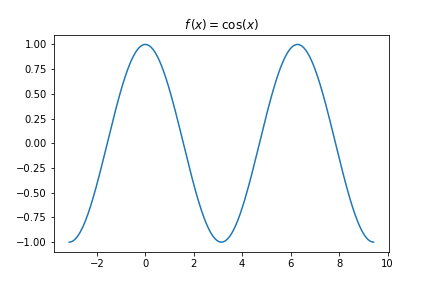
\includegraphics[width=0.8\textwidth]{images/example_graph.png}
    \caption{Image 1}
    \label{fig:1}
\end{figure}

\begin{figure}[ht]
    \centering
    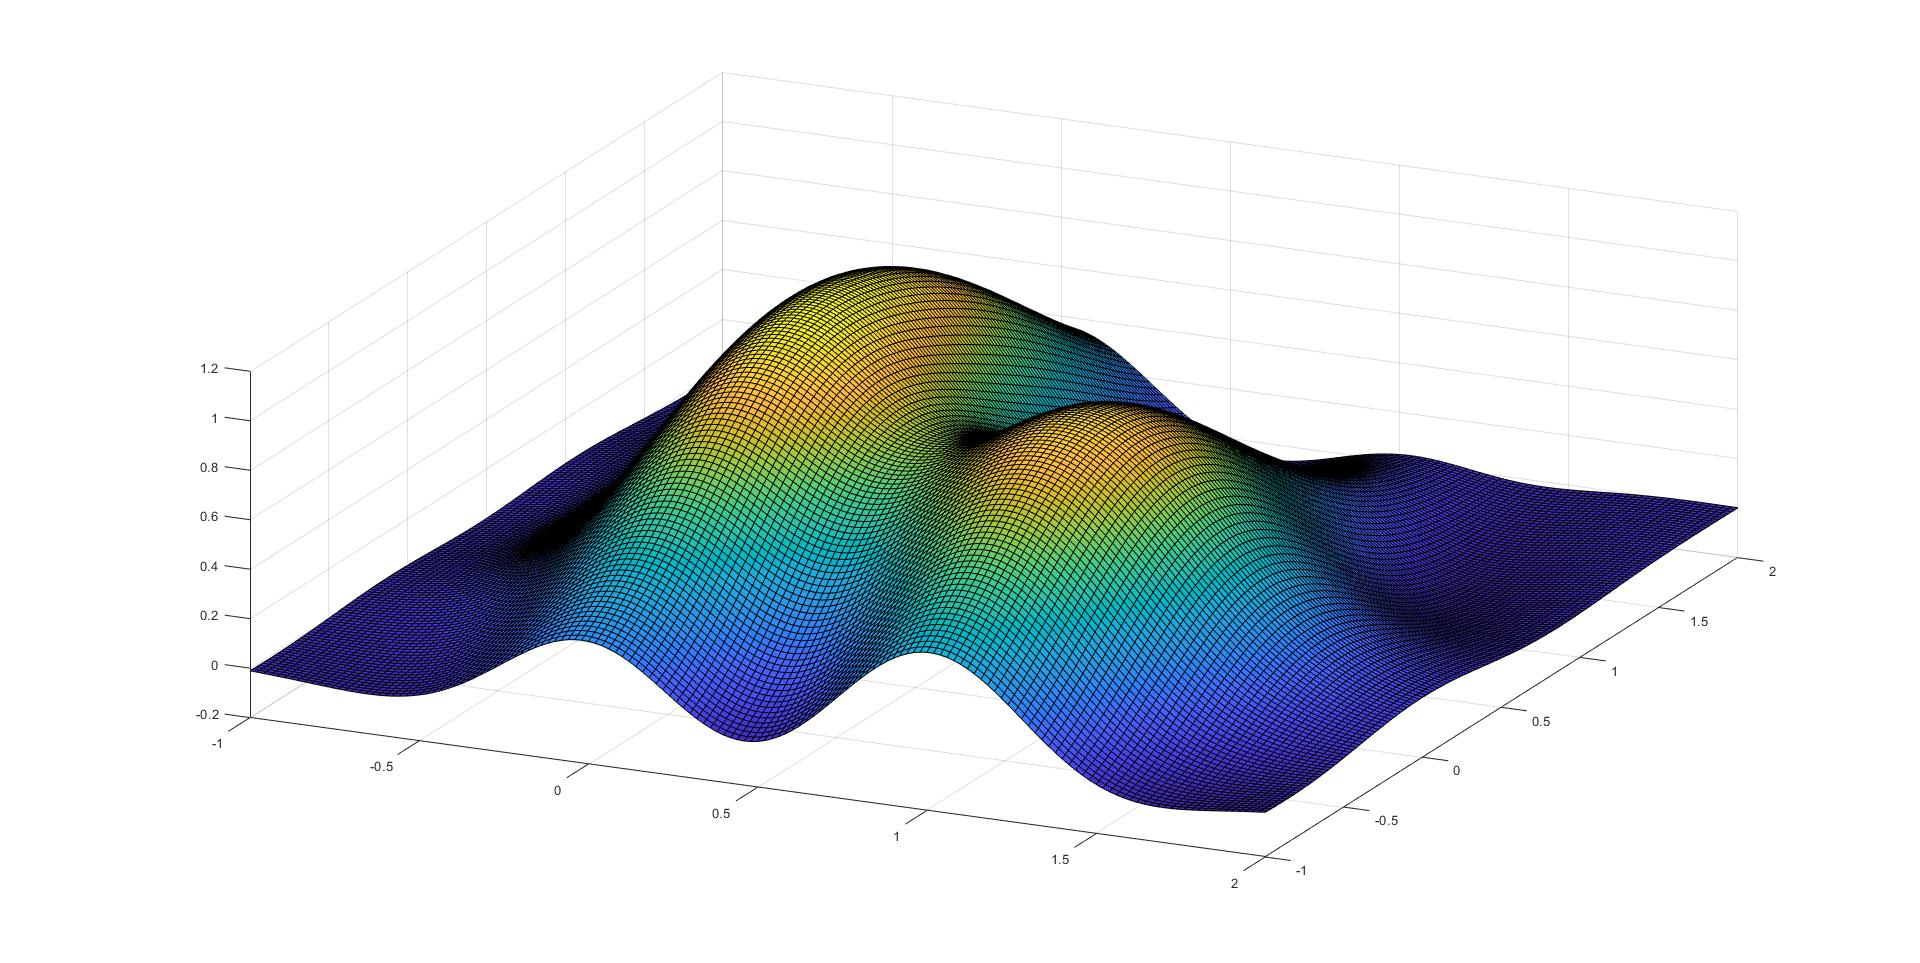
\includegraphics[width=0.8\textwidth]{plot.jpg}
    \caption{Image 2}
    \label{fig:2}
\end{figure}

\newpage

\blindtext
\begin{wrapfigure} {l} {0.5\textwidth} %--- Used for wrapping image around text --- %
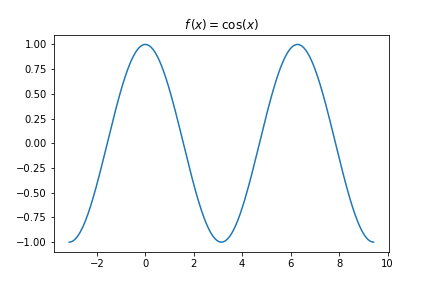
\includegraphics[width=0.5\textwidth]{images/example_graph.png}
\caption{Image 3}
\end{wrapfigure}
\blindtext
\blindtext

\newpage 
\section{Adding References and Links}
Unlike Latex as discussed in \ref{introduction}, Word is user-friend.
\newline You can learn more about Latex on page \pageref{introduction}.
\newline \begin{equation} \label{polynomial-equation}
ax^2 + bx +c.
\end{equation}
Now you can reference the polynomial equation by \eqref{polynomial-equation}.
You can find more information on\href{https://www.overleaf.com/} { Overleaf}.


\section{More Mathematics}
\begin{center}
$\sum_{n=0} ^ {\infty}$ , Basically for sum = n in range of 0 to infinity.
\vspace{4mm}
 \newline $\sum_{n=0} ^ {\infty}\frac{1}{n^2+1}$ , Another Example. 
 \vspace{4mm}
 \newline The above are examples of inline math.
\end{center} 
 
 Display Math Example : 
\[\sum_{n=0} ^ {\infty}\frac{1}{n^2+1}\]
\vspace{4mm}
Integral Functions :
Inline Math : $\int_{0}^1x^2dx$
\vspace{4mm}
\newline Display Math : \[\int_{0}^1x^2dx\]
\vspace{4mm}
\newline Three Integrals : 
Inline Math : $\iiint_{0}^1x^2dx$
\vspace{4mm}
\newline Display Math : \[\iiint_{0}^1x^2dx\]
\vspace{4mm}
\newline Limits : 
\vspace{4mm}

Inline Math: $\lim_{x\to 1}x$
\vspace{4mm}

Display Math: \[\lim_{x\to 1}x\]

More Examples: 

$\max_{n\in \{1,2,3\}}n, \min , \sup ,\inf, \limsup , \liminf $

\newpage
More Examples - Contd : 
\[\max_{n\in\{1,2,3\}}n\]

Multi-line Example:
\begin{multline}
    f(x) = 2x^2 + 4x +3x^3 + 4 + 2x^2 + 4x +3x^3 + 4= 0;
     \vspace{4mm}
\end{multline}
\newline Only useful when equations are long like the above.

\begin{multline*}
    f(x) = 2x^2 + 4x +3x^3 + 4 + 2x^2 + 4x +3x^3 + 4= 0;
     \vspace{4mm}
\end{multline*}

The above is an example of no—reference naming the equation.
\vspace{4mm}

Align Example : 

\begin{align}
     2x+3y+3z+w &= 2 & 3x+4y+1z+0w = 4 \\
\end{align}

\begin{align}
     2x+3y+3z+w &= 2 & 3x+4y+1z+0w = 4 \\
     2x+3y+3z+w &= 2 & 3x+4y+1z+0w = 4
\end{align}

\begin{align} \label{align env}
     2x+3y+3z+w &= 2 & 3x+4y+1z+0w = 4 \\ \notag
     2x+3y+3z+w &= 2 & 3x+4y+1z+0w = 4 \notag
\end{align}

This is referencing the above equation and you can do the same thing for the multi-line as well: \eqref{align env}

 \section{SPACING IN MATHEMATICS:}

 So I'm just going to attach a URL link to the documentation: \href{https://www.overleaf.com/learn/latex/Spacing_in_math_mode}{Spacing in Math Mode}

\section{Math fonts:}
 To make this, you have to be in math mode: $\mathbf{a}$ this is for boldface used for vectors mostly.

 Calligraphy fonts: $\mathcal{T} , \mathcal{C},$ Difference : $C$

 Blackboard bold: $\mathbb{R}$ only works on capital letters. $\mathbb{a}$ example when used on small letters.


Bar and over line : $\Bar{a}$, $\overline{ab}$

Dot over the letter ( time-derivative functions): $\dot f$

Usual  Derivatives: $f''$

\newpage
\section{Matrices and Cases:}
\[
\begin{matrix}
    1 & 2 & 3 \\
    5 & 6 & 7 \\
    8 & 9 & 0
\end{matrix}
\] Must be enclosed in inline or display math.

\[
\begin{vmatrix}
    1 & 2 & 3 \\
    5 & 6 & 7 \\
    8 & 9 & 0
\end{vmatrix}
\] Another Example of a V Matrix used to find a determinant.

\[
|x| = 
\begin{cases}
    x &  \text{for } x > 0 \\
    0 & \text {for } x = 0 \\
    -x & \text{for } x < 0
\end{cases}
\]

\section{Theorems: }

\begin{theorem}
    This is an example of a theorem remember to add package {asmthm} and create a theorem environment.
\end{theorem}

\begin{definition}
    This is an example of a definition.
\end{definition}

To remove the numbering : 

\begin{theorem}
    This is an example of a theorem remember to add package {asmthm} and create a theorem environment.
\end{theorem}

\begin{definition}
    This is an example of a definition.
\end{definition}


\begin{remark} \label{remark}
    This is an example of a remark.
\end{remark}


You can also label them : 
\ref{remark} Calling all remarks.


\section{Numbering and Theoremstyle:}

\begin{theorem}
    This is an example of a theorem remember to add package {asmthm} and create a theorem environment.
\end{theorem}

\begin{definition}
    This is an example of a definition.
\end{definition}

\begin{proof}
This is an example of proof.
\end{proof}

\newpage
\section{Styling with fonts and colours.}

\textbf{Manipulating Text by Bold.}
\vspace{4mm}
\newline
\textit{Manipulating Text By Italic.}
\vspace{4mm}
\newline
\underline{Manipulating Text By Underlining.}
\vspace{4mm}
\newline
Here is some text that can be manipulated {\sffamily manipulated}.
\vspace{4mm}
\newline
Here is some text that can be manipulated {\ttfamily manipulated}.
\vspace{4mm}
\newline
{\small Here} is some text that can be manipulated {\ttfamily manipulated}.
\vspace{4mm}
\newline
{\huge Here} is some text that can be manipulated {\ttfamily manipulated}.
\vspace{4mm}
\newline
Adding Overleaf Reference Guide in its documentation: \href{https://www.overleaf.com/learn/latex/Font_typefaces}{ Font Manipulation}
\vspace{4mm}
\newline
For font styles: This is a dedicated web page that can be used to add custom fonts in overleaf 
\href{https://tug.org/FontCatalogue/}{Font Catalogue}
\vspace{4mm}
\newline
Adding custom fonts means the engine has to be changed from pdfLatex to the necessary engine accordingly.
Tested and verified.
\begin{comment}
   Include packages :
usepackage{fontspec}   -- Adding custom font styles in section 1.17 Refer to section 1.17 --
setmainfont[BoldFont=*Heavy]{QTDoghaus} -- Adding custom font styles in section 1.17 Refer to section 1.17 --Make sure that the font s part of TEXLive. else download the fonts separately upload them to this project and place them namely in a folder called fonts and access them.
and then for this example, you must change the engine to LuaLatex, which is why I'm not doing an example for this as it entirely engulfs the font of the page as well.
\end{comment}
\vspace{4mm}
\newline
Here is an example of adding {\color{blue} blue} and by adding [] to the package xcolor we can also use colours like {\color{OliveGreen} OliveGreen}.
\vspace{4mm}
\newline
For more colours, refer to the documentation of Latex Reference over here: \href{https://www.overleaf.com/learn/latex/Using_colours_in_LaTeX}{ Using colours in Latex.}
\vspace{4mm}
\newline
You can also use custom colours by using this command \textcolor{mynewcolor}{Here} by declaring it in the preamble of the document.
\vspace{4mm}
\newline
You can also use custom colours by using this command \textcolor{nextcolor}{Here} by declaring it in the preamble of the document.
\vspace{4mm}
\newline
The hex colour reference for HTML colour custom can be found in this \href{https://coolors.co/655a7c-ab92bf-afc1d6-cef9f2-d6ca98}{Coolors} site.

\newpage
\section{Citing with BIBTeX}

Text (Normal - Referencing) Bad Type:
\vspace{4mm}
\newline
A good fairy tail can be found in [1]. A good book is the following [2].
\vspace{4mm}
\newline
[1] H.C Anderson \textit{The Little Mermaid}. 1837.
\vspace{4mm}
\newline
[2] M.Shelley. \textit{Frankenstein}. Oxford University Press, 1818.
\vspace{4mm}
\newline
Using Referencing by bib file : 
\begin{itemize}
    \item First create a <name>.bib
    \item Refer to the documentation given below:
    \begin{itemize}
        \item This is one site \href{https://www.bibtex.com/e/entry-types/}{Bib Tex Entry Types}
        \item This is official documentation site \href{https://www.overleaf.com/learn/latex/Bibliography_management_with_bibtex}{Bibliography management with bibtex}
    \end{itemize}
\end{itemize}
Usage : 
\newline
A good fairy tail can be found in \cite{anderson}. A good book is the following \cite{shelly}


\newpage
\section{Optional Arguments in DocumentClass}
This is an example , cannot be viewed in the pdf: //
\begin{comment}
    Usage : \document class[12pt , fleqn (flush left equations), leqno (left equation number),twocolumns (like papers, reports),landscape (landscape mode)]
\end{comment}
\section{The Letter Document Class}
This is an example , cannot be viewed in the pdf: //
\begin{comment}
    \documentclass{letter}
\signature {R.L.Stine}
\address{What sever your address may be}
\begin{letter} {}
\opening {TO whom so may it concern}
 i hope you are doing well.
 \closing{Yours, Faithfully,}
\end{letter}
% -- \end{document} -- %
\end{comment}

\section{Overleaf Templates :}
To save time you can check out already built templates by clicking this link here: \href{https://www.overleaf.com/latex/templates}{Templates}.

\section{Displaying code with Verbatim}
To write a for-lop in Python, you would write it as 
\begin{verbatim}
    for num in range(1,n):
    print (num **2)
\end{verbatim}


\bibliography{biblio} %--- Importing biblio.bib file into main.tex --%
\bibliographystyle{plain} %--- Important : otherwise the referencing is just "?" ---- %

To add Multiple files easily :
\begin{comment}
    \subfile{section1}
\end{comment}


\end{document}
